\documentclass{standalone}
\usepackage{tikz}

\begin{document}

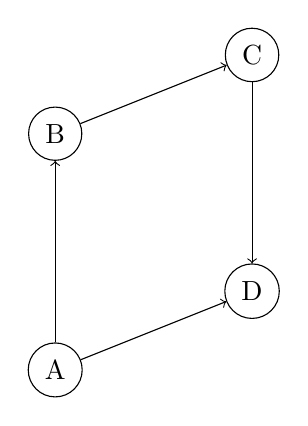
\begin{tikzpicture}
    \node[shape=circle,draw=black] (A) at (0,0) {A};
    \node[shape=circle,draw=black] (B) at (0,3) {B};
    \node[shape=circle,draw=black] (C) at (2.5,4) {C};
    \node[shape=circle,draw=black] (D) at (2.5,1) {D};

    \path [->] (A) edge node[left]   {} (B);
    \path [->] (B) edge node[below]  {} (C);
    \path [->] (A) edge node[below]  {} (D);
    \path [->] (C) edge node[left]   {} (D);
\end{tikzpicture}

\end{document}